\section{Saityno peržiūros sistemų architektūrų apžvalga}

Šiame skyriuje analizuojamos mokslinėje literatūroje aprašytos saityno peržvalgos roboto sistemų realizacijos -- pagrindiniai komponentai, jų funkcinės atsakomybės, charakteristikos, atliekama palyginamoji analizė tarp skirtingų aprašytų realizacijų.

\subsection{Pagrindiniai sistemos komponentai}

M.Najorc ir C. Olston mokslinė saityno peržvalgos sistemų apžvalga (\cite{StanfWebCrawl}) formalizuoja anksčiau literatūroje aprašytas tokių sistemų dizaino specifikas. Joje nusakoma išskirstyto peržvalgos roboto sistemos architektūra -- skirtingose mašinose egzistuojantys žvalgymo procesai, kiekvienas jų turintis keletą lygiagrečiai veikiančių agentų gijų, kurios atlieka kartotinius žvalgymo ciklo žingsius, kuriuose dalyvauja išskiriami pagrindiniai 8 struktūriniai sistemos elementai.

\subsubsection{„Pasienis“}

„Pasienio“ duomenų struktūra (angl. -- \textit{URL Frontier}) saugo URL\footnote{URL - Uniform Resource Locator} adresų sąrašą, kurie bus aplankyti, iš šio sąrašo paduodamas adresas žvalgymo agento gijai pagal atitinkamas žvalgymo mandagumo (angl. -- \textit{Politeness}) ir prioritizavimo (angl. -- \textit{Priority}) politikas. Tai viena iš pagrindinių žvalgymo roboto sistemos būsenos duomenų struktūrų. Jai keliami šie pagrindiniai funkcionalumo reikalavimai:
\begin{itemize}
    \item Pridėti URL adresą į sąrašą
    \item Nuskaityti URL adresą iš sąrašo
\end{itemize}

\subsubsection{HTTP parsiuntimo modulis}

Žvalgymo agentui gavus URL adresą iškviečiamas HTTP modulis, kuris pirmiausia kreipiasi į \textit{DNS adreso išaiškinimo} komponentą tam, jog būtų nustatytas URL resurso serverio vardo IP protokolo adresas \cite{StanfWebCrawl}. Šis veiksmas reikalingas tam, kad būtų minimizuotas HTTP užklausos atsakymo laikas (išvengiama DNS išaiškinimo užklausų į išorinius serverius).

\subsubsection{Saityno nuorodų ištraukiklis}

Šis komponentas (angl. -- \textit{Link extractor}) nuskaito parsiųsto HTML dokumento turinį ir išgauna visas HTML nuorodas tiek į išorinius (angl. -- \textit{offsite links}), tiek į vidinius (\textit{in-site links}) žiniatinklio serverio puslapius.

\subsubsection{Adresų skirstiklis}

Šis modulis (angl. -- \textit{URL distributor}) atsakingas už išgautų nuorodų priskyrimą atitinkamiems žvalgymo procesams.

\subsubsection{Adresų filtras}

Komponentas, kuris filtruoja priskirtus URL adresus ir gali išmesti taisyklių neatitinkančias nuorodas (pvz.: puslapiai įtraukti į juodąjį sąrašą). Taisyklės gali būti specializuotos kiekvienam žvalgymui atskirai.

\subsubsection{Dublikatų šalintojas}

Modulis (angl. -- \textit{Duplicate URL Detector}), kuris saugo visų iki šiol aplankytų nuorodų indikatorius ir praleidžia tik tas nuorodas, kurios anksčiau nebuvo sutiktos. Tai antroji žvalgymo roboto sistemos būsenos dalis (pirmoji -- „pasienio“ komponento žvalgytinų adresų sąrašas), kuriai keliami šie pagrindiniai reikalavimai:

\begin{itemize}
    \item Pridėti URL adreso aplankymo indikatorių į sąrašą
    \item Atlikti URL priklausymo sąrašui testą
\end{itemize}

\subsubsection{Adresų prioritizuotojas}

Komponentas (angl. -- \textit{URL Prioritizer}), kuris kiekvienam URL adresui priskiria tam tikrą prioritetą pagal specializuotus saityno peržvalgos roboto sistemos pasirinkimo politikos faktorius, tokius kaip nustatomas puslapio svarbos laipsnis ar puslapio keitimosi greičio faktorius.


\subsection{Sistemos UML veiklos diagrama}

Atsivelgus į 3.1 poskyrio struktūrinius komponentus pagal \cite{StanfWebCrawl} pasiūlytą schematinį dizainą, galima sudaryti veiklos diagramą, parodančią sistemos ciklinį funkcionavimą.

\begin{figure}[ht]
\centering
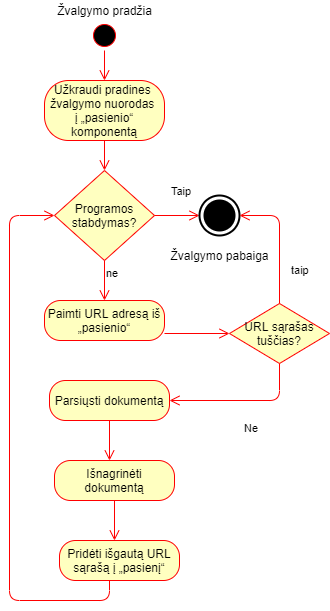
\includegraphics[scale=0.6]{img/Web_Crawler_Activity_Diagram.png}
\caption{Saityno žvalgymo roboto sistemos UML veiklos diagrama \cite{CategoriesOfWebCrawlersAndOverview}}
\label{fig:system_activity_diagram}
\end{figure}

\subsection{Viešai prieinamų realizacijų apžvalga}

Šiame skyriuje apžvelgiamos keletas žinomiausių viešuose akademiniuose literatūros šaltiniuose aprašytų saityno peržvalgos robotų sistemų architektūrų ir siekiama palyginti dizaino sprendimus įvertinant stipriąsias, silpnąsias tokių sistemų puses, rasti bendras šio tipo sistemų komponentes.

\subsubsection{„Mercator“ sistema}

1999 m. išsamiai literatūroje autorių A.Heydon ir M.Najork aprašyta ir eksperimentiškai įvertinta išplečiama, paskirstyta saityno peržvalgos roboto sistemos architektūra. Ši sistema parašyta naudojantis Java programavimo kalba ir jos vykdomąja aplinka (angl. \textit{runtime environment}). Aprašyta sistema didžiąją dalį savo aprašomų duomenų struktūrų talpina disko atmintyje, taip pat nedideli buferiai saugomi operatyvioje atmintyje ir skirti pasiekti greitesnei duomenų prieigai (kešavimo mechanizmas) \cite{MercatorLiterature}.

\subsubsubsection{Žvalgymo agentai}

Sistemoje saityno žvalgymas vyksta naudojant žvalgymo procesų gijas (angl. \textit{worker threads}, kurios veikia lygiagrečiai ir įprastai sistemoje skaičiuojamos šimtais vienetų vienu metu \cite{MercatorLiterature}. Kiekviena gija atsakinga už puslapio atsiuntimą ir apdorojimą (nuorodų suradimą, suabsoliutinimą).

\subsubsubsection{Pagrindiniai sistemos komponentai}

Aprašomos sistemos išsamesnė schema pateikiama šio rašto darbo priede. Šioje dalyje trumpai apžvelgiamos kiekvieno komponento svarbiausios charakteristikos.


\subsubsubsection{„URL siena“}

Šis komponentas (angl. \textit{URL frontier}) saugo visų lankytinų URL adresų sąrašą, sudarytas iš nepriklausomų FIFO (angl. \textit{First-In-First-Out}) principu veikiančių eilių (angl. \textit{queues}), kurių kiekviena priskiriama atitinkam žvalgymo agentui. Taip pat, kai naujas URL adresas pridedamas į kurią nors eilę, konkreti eilė apsprendžiama pagal pridedamo adreso kanoninį vardą (angl. \textit{canonical host name}). Šie du principai įgyvendina žvalgymo roboto sistemos „mandagumo“ politiką -- užtikrinama, jog daugiausiai tik vienas žvalgymo agentas apdoros konkretų saityno serverį, todėl sistema neapkraus žvalgomo serverio resursų.

\vspace{1em}
\textbf{URL adresų saugojimas}
\vspace{1em}

Kadangi saugomas URL adresų sąrašas talpina šimtus milijonų įrašų, nagrinėjamoje sistemoje jie saugomi disko atmintyje, taip pat turimas 600 adresų buferis, saugomas operatyvioje atmintyje ir leidžiantis greičiau apdoroti nuorodas (išimti, idėti).

\subsubsubsection{„HTTP protokolo modulis“}

Peržvalgos robotų sistemos turi atsižvelgti į saityno serveriuose talpinamus \textit{robots.txt} failus, įgyvendinančius REP (angl. \textit{Robots Exclusion Protocol}) ir apibrėžiančius, kokie resursai pateiktame serveryje yra leistini žvalgyti. Aprašomos sistemos HTTP modulis saugo $2^18$ eilės serverio vardo-REP failo kešą.

\subsubsubsection{Įvesties srauto komponentas}


\subsubsection{„PolyBot“ sistemos architektūra}
\subsubsection{„BUbiNG“ didelio masto žvalgymo sistemos architektūra}